\chapter{ELMy H-Modes on C-Mod}\label{ch:Elmy}

The ELMy H-mode \cite{Wagner1982,Keilhacker1984}, described in \cref{sec:hcr_elmy}, is the most commonly-accessed high-performance regime on major tokamak experiments.  The bursty transport driven by ELMs provides sufficient relaxation of the particle confinement in H-mode to allow stationary operation without excessive impurity accumulation; as such, the ELMy H-mode is considered the baseline operating regime for ITER \cite{ITER1999,Shimada2007}.  However, on ITER-scale devices the pulsed heat loading associated with ELMs drives unacceptable levels of erosion and damage to plasma-facing wall and divertor materials \cite{Loarte2003,Federici2003}.

In light of the impact of large, deleterious ELMs on the ITER wall, and the profound impact of pedestal height on overall plasma performance \cite{Kinsey2011,Doyle2007}, a firm understanding of the physics governing the pedestal in high-performance regimes and their extrapolation to reactor-scale devices is of paramount importance to fusion research leading up to ITER operation.  To that end, a Joint Research Target combining theory, experiment, and modeling efforts in the ELMy H-mode pedestal was undertaken \cite{Groebner2013}\gnote{cite tech report too?}.  Notably, this effort saw the development of the EPED model \cite{Snyder2009,Snyder2011,Snyder2009a}, described in \cref{sec:mod_eped}, which predicts the pressure pedestal width and height preceding the ELM crash through a combination of constraints based on peeling-ballooning MHD instability \cite{Snyder2004,Wilson2002,Wilson2006} (\cref{sec:mod_pb}) and kinetic-ballooning turbulence \cite{Snyder2001} (\cref{sec:mod_turbulence}).  In this chapter, we detail the contributions from Alcator C-Mod to this joint effort \cite{Walk2012}\gnote{how to emphasize my own contribution?} both in empirical studies of the ELMy H-mode pedestal, and in the implementation of the EPED model.  The techniques developed in this analysis will subsequently be applied to I-mode pedestals\gnote{reword}.\nicesectionending

\section{ELMy H-Mode Access \& Experimental Arrangement}\label{sec:elmy_access}

\begin{figure}[t]
 \pushtooutside
 \fcapside[55mm]{\caption{C-Mod cross-section comparing the typical plasma shape (blue) to the altered shape favoring ELMy H-mode operation (red), developed in joint experiments with the JFT-2M tokamak \cite{Hughes2013}.  ELMy H-mode access is favored by high lower triangularity and an outer strike point in the divertor slot, coupled with very low upper triangularity and elongation.  This is thought to reduce the required edge pressure gradient and current to reach the peeling-ballooning boundary.}\label{fig:elmy_shaping}}{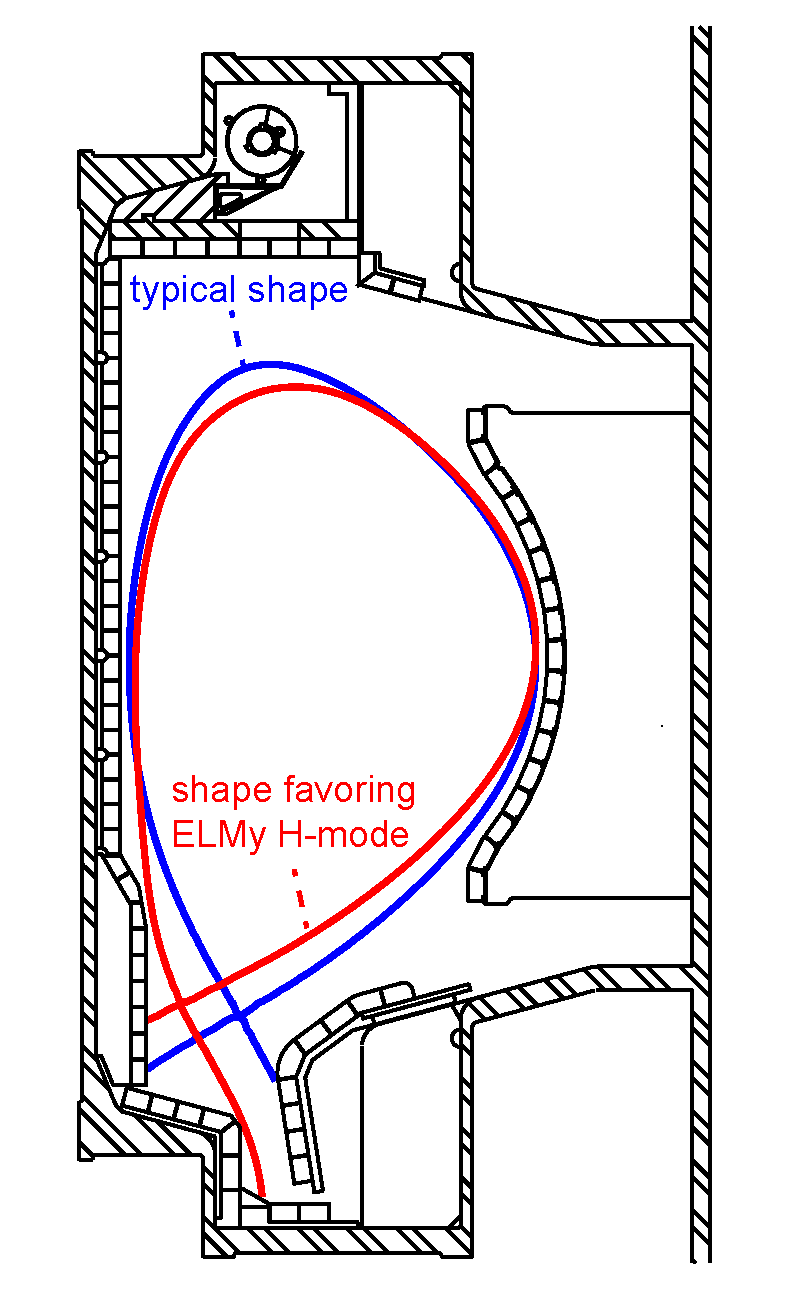
\includegraphics[width=90mm]{graphics/ELMy/shaping.pdf}}
\end{figure}

High-confinement operation on Alcator C-Mod differs is unique among major tokamak experiments in that typical H-modes do not exhibit the large Type-I ELMs\gnote{cite for this?} customarily seen on other devices.  Instead, ELM-free H-modes tend to form at lower collisionalities heating power levels, with high-density, high-power operation tending towards the continuously-regulated EDA H-mode rather than exhibiting discrete ELMs (see \cref{sec:hcr_elmfree,subsec:hcr_eda}).

\nicesectionending

\section{ELM Cycle Synchronization}\label{sec:elmy_sync}

\nicesectionending

\section{EPED Model Predictions}\label{sec:elmy_eped}

\nicesectionending

\section{$I_p$ Scan}\label{sec:elmy_ip}

\nicesectionending

\section{Pedestal Width Scalings}\label{sec:elmy_width}

\nicechapterending

\bibliographystyle{../plainurl}
\bibliography{../references}